\documentclass{article}

\usepackage[T1]{fontenc}

\usepackage[affil-it]{authblk}

\usepackage[USenglish,american]{babel}
\usepackage[pdftex]{graphicx}
\usepackage{epstopdf}

\usepackage{cite}

\usepackage{amsfonts,amsmath,amsthm,amssymb}

\usepackage{tikz,pgf}
\usetikzlibrary{fit}

\usepackage{csvsimple}

%\pagestyle{empty}
\setlength{\parindent}{0mm}
\usepackage[letterpaper, margin=1in]{geometry}
%\usepackage{showframe}

\usepackage{multicol}
\usepackage{enumerate}

\usepackage{verbatim}
\usepackage{listings}

\usepackage{color}

\lstset{%
    language         = Python,
    basicstyle       = \footnotesize\ttfamily,,
    keywordstyle     = \bfseries\color{blue},
    stringstyle      = \color{magenta},
    commentstyle     = \color{red},
    showstringspaces = false,
    backgroundcolor  = \color{lightgray},
    numbers          = left,
    title            = \lstname,
    numberstyle      = \tiny\color{lightgray}\ttfamily,
}

\usepackage{xspace}
\usepackage{url}
\usepackage{cite}

\usepackage{titlesec}
\titlespacing*{\subsubsection}{0pt}{*0}{*0}
\titlespacing*{\subsection}{0pt}{0pt}{*0}
\titlespacing*{\section}{0pt}{0pt}{*0}

\newcommand{\Bold}{\mathbf}

\setlength{\parskip}{1em}
%\setlength{\parindent}{1em}

\title{Expert Modeling System}
\date{\today}
\author{Philip Robinson}
\affil{NASA: Jet Propulsion Laboratory}

\begin{document}

\maketitle

\begin{abstract}
  In a large community, enlisting potential collaborators and subject matter experts
  greatly impacts the success of projects. Candidate discovery and expertise ranking
  against a task or project is necessary to inform recruiting
  of impactful teams\cite{Minto2007}. NASA's Jet Propultion Lab is interested in
  better tools for expert discovery and matchmaking
  to tasks in misssion critical, late stage, anomalies.
  Topic modeling, such as Biterm Topic Model (BTM)\cite{Yan2013,Chen2015}, Latent
  Dirichlet Allocation (LDA),
  and Correlated Topic Model (CTM), have long been used to as discovery tools,
  usually focused on exploratory analysis, finding topics for text\cite{Alghamdi2015}.
  Likewise,
  author modeling has been used to measure attribution\cite{Rexha2018} and
  contribution\cite{AldebeiHJ016}. Author-Topic Modeling (ATM) establishes a strategy to
  map both authors and documents to the same topic-space over a vocabulary\cite{RosenZvi2004}.
\end{abstract}

% http://www.sfp.caltech.edu/students/proposal/other_project_plans
% https://trs.jpl.nasa.gov/

\begin{multicols}{2}

\section{Introduction}

Building effective teams, especially against specialized projects, is essential to project
success. With a greater candidate pool, matchmaking often falls on managers whose scope is
socially limited.
In order to best
support the scale of an institution like JPL/NASA, and domain specific
nature of the problems they address, they are
interested in strategies to explore and recommend subject matter experts (SME). An
effective SME recommender system
significantly reduces social coordination overhead of electing contributors to
to complex, domain specific, problems. Additionally, tools that allow exploratory
and comparative view of experts have potentially great benefits to workload
balancing and identifying company knowledge gaps.

Latent Dirichlet Allocation (LDA) is a topic modeling strategy that empowers
exploratory analysis, topic discovery, and dimmensionality reduction.
Since we are looking for SMEs,
author-modeling is a closer fit. The phrase ``author modeling'' has also been used
in techniques which are more concerned with literal text-content document
contribution and attribution\cite{Rexha2018}; we are not interested in these techniques.
Although LDA is best used as an exploratory tool, many derivatives exist that
leverage LDA for more powerful or specific applications.
One extension to LDA is the author-topic model, which attempts to describe authors in
LDA's learned topic space.


\section{Objectives}

The Jet Propulsion Lab uses a ticketing system called the Problem Reporting System
to manage work assignment of experts to mission critical late stage anomalies.
This ticketing system contains Pre-Launch Failure Reports (PFR)s and
Incident Surprise Anomalies (ISA)s. Without an expert assignment strategy,
candidates are usually elected by the manager of a ticket, which is susceptible to bias
of their prior collaborators, may require understanding of candidate skills beyond their
purview, and usually leads to over assigning tickets to few candidates.
Better management of human resources by exploratory tools and recommender systems,
would significantly reduce the difficulty of building
effective teams.
%In addition to developing clustering and comparison strategy,
%a full, usable, search prototype for use by the Mission Risk Assessment (5X) team.

\section{Method}

Traditionally, in representing a document collection, we envision a
\[\texttt{Vocabulary Size x Document Count} \]
matrix. This is a very high dimensional structure.
In order to effectively
traverse this corpus, we hope to express documents in the form of principle components,
a dimmensionality reduction technique that strictly describes an observed document
set. This can be very difficult to interpret and has very little predictive power for
unobserved documents.

Latent Dirichlet Allocation is a generative model for fitting topics to a corpus.
This is done by electing a document, then a topic for that document, then a word for that topic.
The yield of this trained model is a mapping from an input document to a topic-space.
This is a softer definition allowing us to observe future documents.

The Author-Topic-Model extends LDA to model authors as a mixture of topics. This is,
again, a generative model that elects a document, then an author for that document,
then a topic for that author, then a word for that topic. This still learns a topic space
from the vocabulary, but expresses both authors and documents in this topic space.

For the PRS, persons who are assigned to tickets are considered experts in that topic, because
they are able to or have resolved that ticket. In this implementation the assignee is expressed
as an author. This process results in a dimmensionality reduction over our topic space, and
an inferred dimmensionality increase for our authors (who were previously just singleton tokens).

\section{Fitting}

As long as these authors are appropriately represented in the training set, they act as
a strong litmus test against this author modeling technique. This is difficult to replicate,
due to the small sparse candidate dataset, so we explore rank utility\cite{Gunawardan,Silveira2017}
instead.

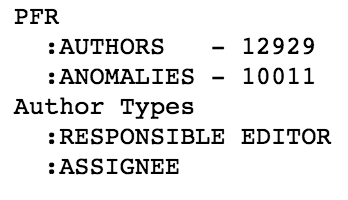
\includegraphics[width=.27\columnwidth]{../images/PFR_count.png}
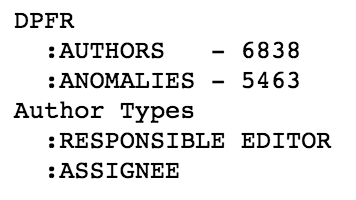
\includegraphics[width=.27\columnwidth]{../images/DPFR_count.png}
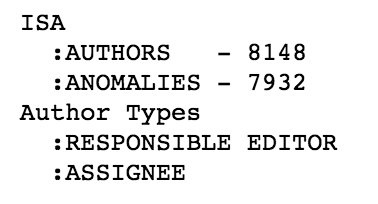
\includegraphics[width=.27\columnwidth]{../images/ISA_count.png}

They\cite{RosenZvi2004}
also state and describe the process for using these single author papers for perplexity.
\begin{quote}
  Perplexity is the standard measure for estimating the performance of a probabilistic model.
\end{quote}
Alternative, exploration using coherence metrics\cite{Roder2015}, as this has been shown to
provide more understandable topics when applied to bag-of-words topic models.

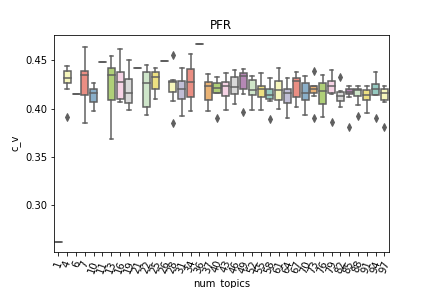
\includegraphics[width=\columnwidth]{../images/PFR_c_v.png}
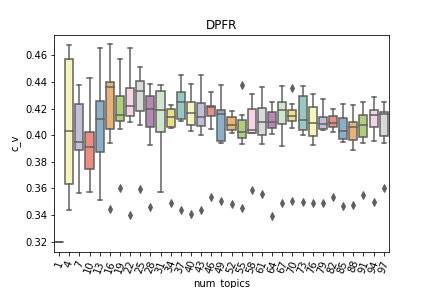
\includegraphics[width=\columnwidth]{../images/DPFR_c_v.png}
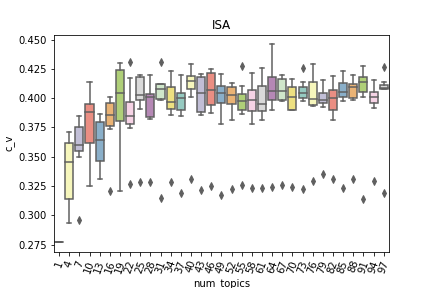
\includegraphics[width=\columnwidth]{../images/ISA_c_v.png}

It is worth asking if number of publications impacts model performance,
in unexpected ways. From the plots below it is shown that the predictive power
does not significantly deviate with publication count.

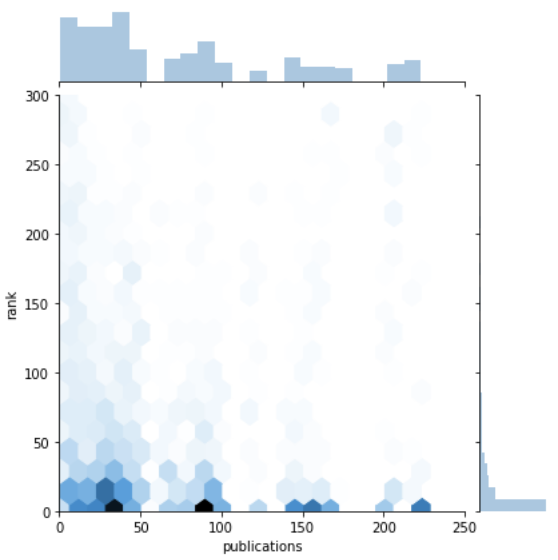
\includegraphics[width=\columnwidth]{../images/Test_pubs.png}
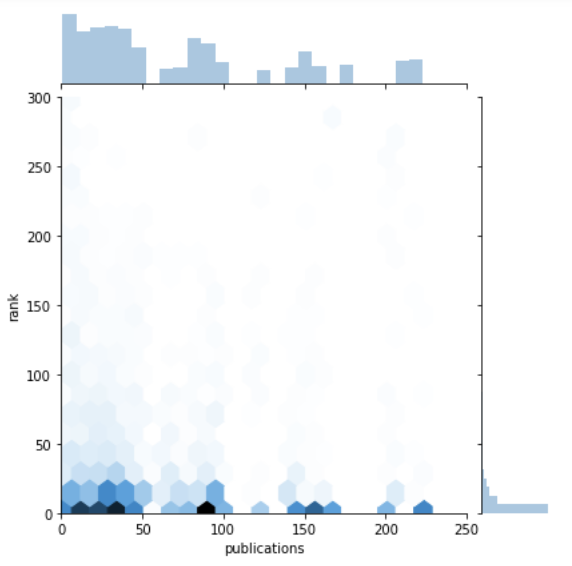
\includegraphics[width=\columnwidth]{../images/Train_pubs.png}

It is also interesting to know how much text is required to inform
our model prediction. For these plots, we randomly subset texts for
known ticket-expert pairs and observe the expert's new ranking. It is
shown that at 30 words, our model is considered consistent with best fit.
This is significantly less than our average document size.

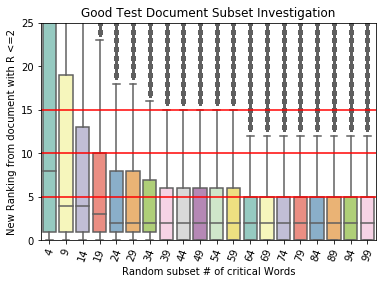
\includegraphics[width=\columnwidth]{../images/low-ranked-downsample.png}
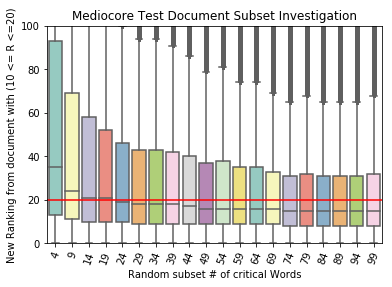
\includegraphics[width=\columnwidth]{../images/mid-ranked-downsample.png}

Finally, its important to look at predictive power. These plots show the
recall from the top 15 elements for \texttt{ISA} documents over \texttt{train}
and \texttt{test}.

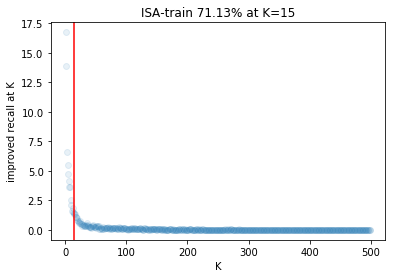
\includegraphics[width=\columnwidth]{../images/recall-train-isa.png}
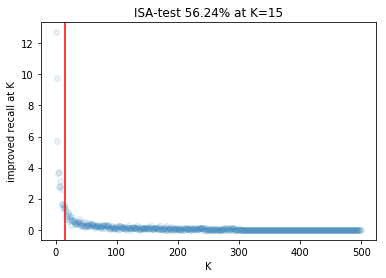
\includegraphics[width=\columnwidth]{../images/recall-test-isa.png}


%In my original proposal I suggested an informed train test split by bisecting with
%min-cut\cite{Feige2002} a graph where authors are vertices, and edges exist for each
%co-authors relationship, and is labeled by document name. Unfortunately our dataset was
%had to few co-attributions to support this.

%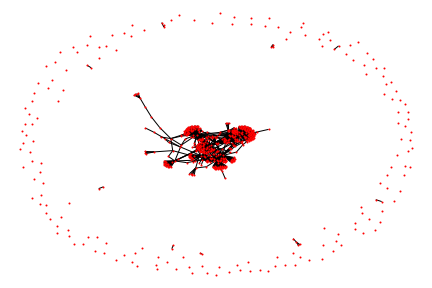
\includegraphics[width=\columnwidth]{../images/PFR_authorship_graph.png}
%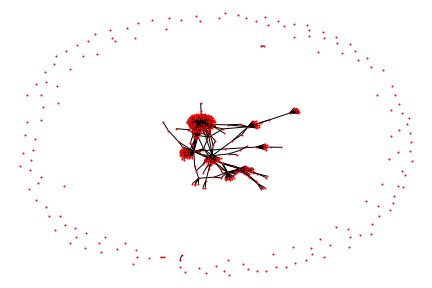
\includegraphics[width=\columnwidth]{../images/DPFR_authorship_graph.png}
%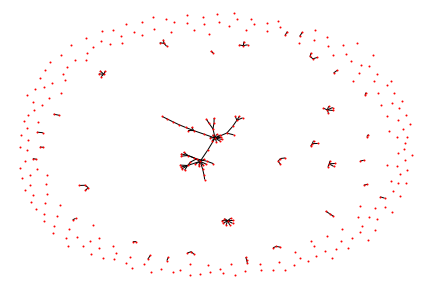
\includegraphics[width=\columnwidth]{../images/ISA_authorship_graph.png}

\section{Results}

The yield of this project is a site to allow queries against a learned
model. This will be used to beta test and gather more data from customers
using the 5x PRS.


\includegraphics[width=\columnwidth]{../images/site-demo.png}

The application goals are met sufficient to move this project
forward, and incorporate more data.
It will also be important that we investigate the stability of
models\cite{Yang2016}, in order
to incorporate later documents, while minimizing effect to the user
experience. Finally, we need to better understand our false positives.
This will require contacting persons who rank high but are not attributed
to those tickets.


\section{Acknowledgments}

I want to thank Ian Colwell, Valentinos Constantinou, Chris Mattman, Jerry Chen, Leslie Callum, Bruce Waggoner, and Harald Schone for acting as guides and resources through this project. This was a lot of fun. I feel we all did something pretty cool here.

\bibliography{references.bib}{}
\bibliographystyle{plain}
\end{multicols}

\end{document}
